\chapter{Developer Documentation} % Developer guide
\label{ch:impl}
This chapter covers the developer’s Manual, which contains the basics and process of development. Initially, a detailed specification of the project is explained. In order to present the usage of the APIs, a brief overview of HTTP requests, their URI locations, and response structures are described. Afterwards, the developer is introduced to main components, storing, and updating models in PostgreSQL, and communication with Kubernetes. Finally, the testing plan and results of the tests are given.

\section{Prerequisites}
Before writing the code, the developer must have a few necessary tools. The installation links can be found in references.
\begin{itemize}
    \item Project available from GitHub~\cite{mini-eo-cm}
    \item PostgreSQL~\cite{postgresql-download}
    \item Postman~\cite{postman}
    \item IntelliJ IDEA development environment~\cite{intellij-idea}
\end{itemize}

\section{Specification}
\label{sec:specification}
This section will specify all the features of the project. Since the unknown user cannot enter the application, the use case diagram in~\autoref{ssec:figure-for-life-cycle-application} is explained from the user and admin point of view.

If the user does not have an account, he must register to the system.
After registering the user is able to do 3 kinds of management. These are Package, Resource, and Kubernetes management. After creating a package the user is able to create the resource. By creating a resource, the YAML file is uploaded to the application which later on can be deployed into Kubernetes. Packages can be deleted and updated, YAML files that have been uploaded can be read and deleted, and lastly deployed namespace can be deleted from Kubernetes. 

Admin has special credentials to log in to the system. After being able to log in, the list of users is visible. The users can be deleted by the admin as well.

\begin{figure}[H]
	\centering
	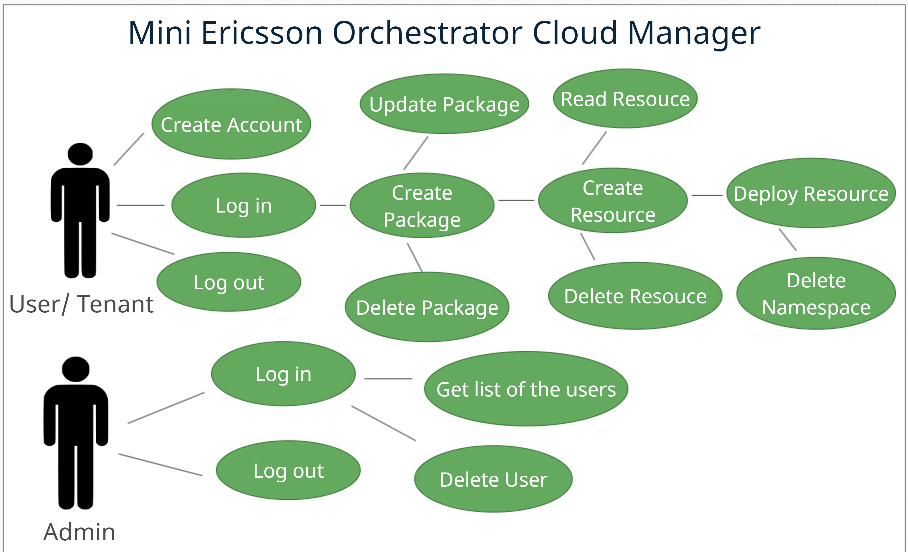
\includegraphics[width=\textwidth]{images/use-case-diagram-3.png}
	\caption{Use case diagram of the application}
	\label{ssec:figure-for-life-cycle-application}
\end{figure}
So far we have seen the overview of what our application is capable of doing. In the next section, all of these components are explained in detail.

\label{sec:implementation}
\section{Implementation}
This section describes how HTTP requests, which are developed by Spring boot, communicate with the front-end tool and database, including how to manipulate data and use models to update the database. Implementation of the Kubernetes API with the usage of the client library is detailed. Then the background of the encryption of the passwords and authentication of the REST APIs are presented from the developer's point of view.

\label{subsec:api-overview}
\subsection{API overview}
Mini Ericsson Orchestrator Cloud Manager employs the Representational State Transfer (REST) architectural style. All the API operations use the JavaScript Object Notation (JSON) lightweight data-interchange format. The operations use these HTTP verbs:
\begin{enumerate}
    \item GET\\
    Queries for a list of items or for details on a single item. For example, \texttt{getUserPackages}, \texttt{getUserResources} or \texttt{getUsers}.
    \item POST\\
    Requests that create or logging in, out to the system. For example, \texttt{createPackage}, \texttt{createResource} or \texttt{login}.
    \item PUT
    Request that modify a package, resource. For example, \texttt{updatePackage}.
    \item DELETE
    Requests that delete a service such as package, user. For example, \texttt{deletePackage}, \texttt{deleteResource} or \texttt{deleteUser}.
\end{enumerate}

\subsubsection{URI Location}
The Uniform Resource Identifier (URI) location resides in the \texttt{packageManager} directory on the Mini Ericsson Orchestrator Cloud Manager host URL. For example to access the order operations enter the URL: http://localhost:8080/packageManager. The verb and the values in the URL determine which operation is executed. This example shows \texttt{packageList} operation.

\lstset{caption={Mini Ericsson Orchestrator Cloud Manager API URL}, label=src:get-api-example}
\begin{lstlisting}[language={XML}]
GET
http://localhost:8080/packageManager/packageList
\end{lstlisting}

\subsubsection{General Request Headers}
All inbound requests include a general-header section. For authentication, the header must have an Authorization. The system validates Authorization before it processes a request.

If a POST or PUT operation requires a request body, the header must also include the \emph{Content-Type} property. The \emph{Content-Type} property must be set to \emph{application/json} 

\subsubsection{Authorization}
To send the username and password authentication for every request, use the \texttt{Authorization} property. In this case, the user credentials are Base63 encoded.

\lstset{caption={Request Header}, label=src:request-header-example}
\begin{lstlisting}[language={XML}]
Authorization: Basic <encoded credentials>
Content-Type: application/json
\end{lstlisting}

- <encoded credentials> - ASCII Base64 encoding of the credentials in the format "username:password".

\subsubsection{Response Body Structures}
\label{subsubsec:response-body-structures}

The response includes a status and entity schema. If the response is successful, then the \texttt{status} and \texttt{requestStatus} is equal to \texttt{200} and \texttt{SUCCESS} respectively. Otherwise \texttt{404} and \texttt{ERROR} are the  values for \texttt{status} and \texttt{requestStatus}.

\lstset{caption={Success response example}, label=src:success-response-example}
\begin{lstlisting}[language={Xml}]
{
    "status": 200,
    "entity": {
        "requestStatus": "SUCCESS",
        "messages": [
            {
                "msgText": "Username with 'admin' is authorized!"
            }
        ]
    }
}
\end{lstlisting}
\lstset{caption={Error response example}, label=fig:error-response-example}
\begin{lstlisting}[language={Xml}]
{
    "status": 404,
    "entity": {
        "requestStatus": "ERROR",
        "messages": [
            {
                "msgText": "We couldn't find username with 'Kanan' in the system!"
            }
        ]
    }
}
\end{lstlisting}

\subsection{Models}
\label{subsec:models}
There are SQL scripts \texttt{data.sql} and \texttt{schema.sql} where tables are created and objects can be inserted or deleted when the application starts running.

\lstset{caption={\texttt{schema.sql} file}, label=src:schema-sql}
\begin{lstlisting}[language={SQL}]
CREATE TABLE package(
 id varchar(100) NOT NULL,
 name varchar(100) NOT NULL,
 type varchar(100) NOT NULL,
 creationTime TIMESTAMP NOT NULL DEFAULT CURRENT_TIMESTAMP,
 updatedTime TIMESTAMP NOT NULL DEFAULT CURRENT_TIMESTAMP,
 username varchar(100) NOT NULL,
 PRIMARY KEY (id));

CREATE TABLE users(
 username varchar(100) NOT NULL,
 password varchar(100) NOT NULL,
 role varchar(100) NOT NULL,
 lastEnteredTime TIMESTAMP,
 PRIMARY KEY (username));

CREATE TABLE resources(
 id varchar(100) NOT NULL,
 name varchar(100) NOT NULL,
 kind varchar(100) NOT NULL,
 available boolean NOT NULL,
 username varchar(100) NOT NULL,
 PRIMARY KEY (id));
\end{lstlisting}

\lstset{caption={\texttt{data.sql} file}, label=src:data-sql}
\begin{lstlisting}[language={SQL}]
insert into users(username, password, role, lastEnteredTime) values('admin','Qr6AgNbWILBmh7UBoHkEJHUH7TVd2eCpgFtB7csx7ABOW2NbOh4xU0WoAHp0oFN5','admin', null);
\end{lstlisting}

Because \texttt{data.sql} file contains an insertion of \texttt{admin} user, we can enter an admin role to the application without even registering. 

\texttt{src/main/java/com/ericsson/packageManager/entity} is a folder that contains all the necessary model classes to make these objects capable of interacting with a database. As we know, each model is represented by a Java class.

\subsubsection{User}
User is a model in Mini EO-CM application for the authentication system. Basically, it represents the tenants and admins who interact with our project and handle user accounts and authentications. Each user has a username, password, role, and last entered time.

\subsubsection{Package}
Packages can be created by providing Package type and Package name. There are 5 fields for Package to cooperate with other models. These are \texttt{ID}, \texttt{Name}, \texttt{Type}, \texttt{CreationTime}, \texttt{UpdatedTime} and \texttt{Username}. Here \texttt{ID} is the primary key element. Universal Unique Identifier (UUID) is used to uniquely identify a package. Information about the UUID can be found on the website~\cite{uuid-id}.

\subsubsection{Resource}
The Resource model has the following attributes: \texttt{ID}, \texttt{Name}, \texttt{Kind}, \texttt{Available} and \texttt{Username}. \texttt{Resource ID} describes which package it belongs to. \texttt{Kind} shows what type of YAML file has been uploaded while \texttt{Available} field indicate whether resource has been deployed to Kubernetes or not.

\subsection{React Js - Spring}
\label{subsec:reactjs-spring}

React Js communicates with the Spring Boot application with the help of \texttt{fetch} methods. By using different methods of request (POST, PUT, DELETE, GET), URL and content, Spring Boot gets the request, executes the command accordingly, and returns the appropriate response. This response is rendered in React Js and printed out to the screen.

POST request below for creating a Package is described below. Name and type variables are called from input fields. Based on them, a new attribute containing both is initialized. This attribute is converted into JSON format, and it is included in content when fetching that request. URL and request type is specified as well. The response transformed into a readable JSON file. By using new \texttt{res} attribute, we can get \texttt{responseCode}, \texttt{requestStatus} and \texttt{message}.
\lstset{caption={POST request via React Js}, label=src:post-request-js}
\begin{lstlisting}[language={Java}]
        const pac={name, type}
      fetch("packageManager/createPackage",{
        method:"POST",
        headers:{"Content-Type":"application/json"},
        body:JSON.stringify(pac)
      }).then((response) => response.json()).then((res) => {
          let requestStatus = user.entity.requestStatus
          let message = user.entity.messages[0].msgText
      })
\end{lstlisting}

Another example illustrates a GET request to obtain all the packages as a list. For this \texttt{useState} is used in order to store those elements. As usual, URL, HTTP request type is included for \texttt{fetch} request. The result was first converted into readable JSON, afterwards, it was assigned to \texttt{packages} variable using \texttt{setPackage} method. This \texttt{packages} will be used subsequently in displaying. \texttt{useEffect} hook allows you to perform side effects in your components. Here, fetching the data, and directly updating the DOM are all included.
\lstset{caption={GET request via React Js}, label=src:get-request-js}
\begin{lstlisting}[language={Java}]
    const[packages,setPackages] = useState([])
    useEffect(()=>{
      fetch("packageManager/userPackageList").then(res=>res.json()).then((result)=>{
        setPackages(result);
      })
    },[])
\end{lstlisting}

\subsection{Interaction with Database}
\label{subsec:interaction-db}

Spring Boot project connects to a data source using configurations to the one shown below in the project’s \texttt{application.properties} file. These configurations give Spring Boot access to a PostgreSQL database. 

\lstset{caption={\texttt{application.properties}}, label=src:app-properties}
\begin{lstlisting}[language={XML}]
spring.datasource.url=jdbc:postgresql://localhost:5454/postgres
spring.datasource.username=postgres
spring.datasource.password=postgres
\end{lstlisting}

The next part is about how Packages can be inserted, updated, listed, or deleted from the database using SQL statements in Java.

\subsubsection{Insertion}
The JDBC template is the core API through which accessing most of the functionalities is possible such as running statements, procedure calls, and iterating over the \texttt{ResultSet} and returning objects. Since Package has named parameters, the \texttt{NamedParameterJdbcTemplate} framework for JDBC template can be used.

Initially, an SQL statement is created with column names. Using the \texttt{MapSqlParameterSource} we can provide all the values for the named parameters. Afterwards, \texttt{update} method is executed.

\lstset{caption={\texttt{insertPackage} method}, label=src:insert-java}
\begin{lstlisting}[language={Java}]
public String insertPackage(Package aPackage) {
    final String sql = "insert into package(id, name, type, creationTime, updatedTime, username) values(:id,:name,:type,:creationTime,:updatedTime,:username)";
    
    KeyHolder holder = new GeneratedKeyHolder();
    SqlParameterSource param = new MapSqlParameterSource()
        .addValue("id", aPackage.getId())
        .addValue("name", aPackage.getName())
        .addValue("type", aPackage.getType())
        .addValue("creationTime", new Timestamp(System.currentTimeMillis()))
        .addValue("updatedTime", new Timestamp(System.currentTimeMillis()))
        .addValue("username", aPackage.getUsername());
    template.update(sql,param, holder);
}
\end{lstlisting}

\subsubsection{Modification}
\texttt{updatePackage} is a bit different from \texttt{insertPackage}, because Package with \texttt{ID} already exists. Therefore just changing SQL statement is enough.

\lstset{caption={\texttt{updatePackage} method}, label=src:update-java}
\begin{lstlisting}[language={Java}]
public void updatePackage(Package aPackage) {
        final String sql = "update package set name=:name, type=:type, updatedTime=:updatedTime, username=:username where id=:id";

        KeyHolder holder = new GeneratedKeyHolder();
        SqlParameterSource param = new MapSqlParameterSource()
                .addValue("id", aPackage.getId())
                .addValue("name", aPackage.getName())
                .addValue("type", aPackage.getType())
                .addValue("updatedTime", new Timestamp(System.currentTimeMillis()))
                .addValue("username", aPackage.getUsername());
        template.update(sql,param, holder);
    }
\end{lstlisting}

\subsubsection{Deletion}
By providing Package ID and creating a SQL statement will be followed by \texttt{executeUpdate} method. This should be done \texttt{PreparedStatementCallback} because a single \texttt{executeUpdate} call or repeated \texttt{executeUpdate} calls with varying parameters must be executed there.

\lstset{caption={\texttt{deletePackage} method}, label=src:delete-java}
\begin{lstlisting}[language={Java}]
public void deletePackage(Package aPackage){
        final String sql = "delete from package where id=:id";

        Map<String, Object> map = new HashMap<String, Object>();
        map.put("id", aPackage.getId());

        template.execute(sql, map, new PreparedStatementCallback<Object>() {
            @Override
            public Object doInPreparedStatement(PreparedStatement ps)
                    throws SQLException, DataAccessException {
                return ps.executeUpdate();
            }
        });
    }
\end{lstlisting}

\subsubsection{Get}
\texttt{RowMapper} interface is used for querying results to Java objects. For every row returned by the query, Spring uses the row mapper to generate the Java bean.
\lstset{caption={\texttt{findAll} method}, label=src:get-java}
\begin{lstlisting}[language={Java}]
public List<Package> findAll() {
        return template.query("select * from package", new PackageRowMapper());
    }
\end{lstlisting}

\lstset{caption={\texttt{mapRow} method}, label=src:map-java}
\begin{lstlisting}[language={Java}]
public Package mapRow(ResultSet rs, int arg1) throws SQLException {
        Package aPackage = new Package();
        aPackage.setId(rs.getString("id"));
        aPackage.setName(rs.getString("name"));
        aPackage.setType(rs.getString("type"));
        aPackage.setCreationTime(rs.getTimestamp("creationTime"));
        aPackage.setUpdatedTime(rs.getTimestamp("updatedTime"));
        aPackage.setUsername(rs.getString("username"));

        return aPackage;
    }
\end{lstlisting}

The same logic is also applied to Resource and User models. So far we have learned how packages are stored in the database, and how SQL statements are sent to the PostgreSQL to update or delete the package. Now we can dive into the implementation of the file uploading.

\subsection{File management}
\label{subsec:file-management}

In this section, we aim to observe how YAML files are getting uploaded and stored. First of all, when the application starts running, \texttt{resources} folder gets created in the root directory.
\lstset{caption={Bean to create \texttt{resources} folder}, label=src:bean-create-folder}
\begin{lstlisting}[language={Java}]
    @Bean
    CommandLineRunner init(StorageService storageService) {
        return (args) -> {
            storageService.init();
        };
    }
    //
    public void init() {
        Files.createDirectories(rootLocation);
    }
\end{lstlisting}

We need to register a \texttt{MultipartConfigElement} class to upload files with Servlet containers. It is auto-configured in Spring Boot.

\lstset{caption={\texttt{createResource} method}, label=src:create-resource-file}
\begin{lstlisting}[language={Java}]
@PostMapping("/{id:.+}")
public Response createResource(@PathVariable String id, @RequestParam("file") MultipartFile file, @RequestParam("kind") String kind) {
    //
    storageService.store(id, file, user.getUsername());
    //
}
\end{lstlisting}

Based on username and Package ID nested folders are created, if there exists one already it will be replaced. Default name for the file will be \texttt{package.yaml}. After the directories and file is created, the content of the original file is copied into the new one.
\lstset{caption={Storing a file}, label=src:store-yaml-file}
\begin{lstlisting}[language={Java}]
    try {
        new File(this.rootLocation.toString() + "\\" + username + "\\" + id).mkdirs();
        Path destinationFile = this.rootLocation.resolve(username).resolve(id).resolve(Paths.get("package.yaml")).normalize().toAbsolutePath();
        try (InputStream inputStream = file.getInputStream()) {
            Files.copy(inputStream, destinationFile, StandardCopyOption.REPLACE_EXISTING);
        }
    } catch (IOException e) {
        throw new StorageException("Failed to store file.", e);
    }
\end{lstlisting}

As you can see in the figure below \texttt{package.yaml} has been created in nested David's folder and Package ID folder. If David creates a new Resource with a different Package ID, a new folder under the David folder will be added.
\begin{figure}[H]
	\centering
	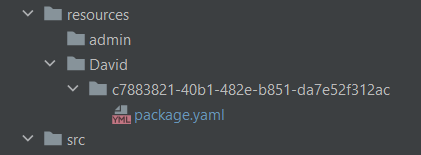
\includegraphics[width=120mm]{images/folder-resources.png}
	\caption{Example Resources Folder}
	\label{ssec:exampple-resource-folder}
\end{figure}

Files can be deleted as well, in this case, both relevant \texttt{package.yaml} and the Package ID folder are deleted. When the admin removes the tenant, the folder related to that user is deleted automatically.

\subsection{Kubernetes-Spring}
\label{subsec:kubernetes-spring-2}

The API server is the core of the Kubernetes control plane. Clusters and external components communicate with each other using HTTP API. Pods, Nodes, and Namespaces are queried and their status can be changed. The kubectl command-line interface is a classic way for operating such requests. However, the possibility of accessing API directly using REST calls leads us to client libraries.

Officially-supported \texttt{Java Kubernetes client library}~\cite{java-k8s-client-lib} often handle common tasks. The library added to the project as well. It can be found in \texttt{lib/java} folder. The following part describes deploying and deleting namespace APIs.

Initially, we should create the \texttt{ApiClient} and then the API stub instance.  \texttt{Service} resources are part of the  \texttt{CoreV1 API}, hence  \texttt{CoreV1Api} instance is created, which will be used to invoke the cluster's API server. As a next step, we instantiate a  \texttt{V1Service} instance based on the YAML file. Consequently, the process of filling all the properties is done. 

Lastly, the API stub that is created should be called. This serializes our resource object and POST the request to the server. \texttt{V1Service} object contains \texttt{metadata} and \texttt{status} fields. Its \texttt{status} field can be checked when it is finished.
\lstset{caption={Create Service Namespace}, label=src:create-service-k8s}
\begin{lstlisting}[language={Java}]
    ApiClient client = Config.defaultClient();
    Configuration.setDefaultApiClient(client);
    //
    Yaml yaml = new Yaml(new Constructor(V1Service.class));
    V1Service yamlSvc = (V1Service) yaml.load(inputStream);

    CoreV1Api api = new CoreV1Api();
    V1Service createResult = api.createNamespacedService("default", yamlSvc, null, null, null);
    //
\end{lstlisting}

Regarding the deletion, \texttt{deleteNamespacedService} method is used to remove the service using default options for this specific kind of resource. The developer can use the last parameter - \texttt{V1DeleteOptions} to specify a grace period and cascading behavior for any dependent resources.
\lstset{caption={Delete Service Namespace}, label=src:delete-service-k8s}
\begin{lstlisting}[language={Java}]
    ApiClient client = Config.defaultClient();
    Configuration.setDefaultApiClient(client);
    //
    try {
        CoreV1Api api = new CoreV1Api();
        V1DeleteOptions body = new V1DeleteOptions();
        api.deleteNamespacedService(getName(id), "default", null, null, 56, true, null, body);
    } catch (ApiException e){
        return ErrorResponse("Service deletion was not succeed");
    }
    //  
\end{lstlisting}

Job workload resources are part of the \texttt{Batch API} while the rest (\texttt{Deployment, ReplicaSet, ControllerRevision, StatefulSet}) are using \texttt{Apps API}.

Here the manipulation between Kubernetes resources and the Java Kubernetes API library has been explained.

\subsection{Jasypt}
\label{subsec:jasypt}

\texttt{Jasypt} is a java library that allows the developer to add basic encryption capabilities to projects with minimum effort. It is also useful for people who do not have deep knowledge of cryptography. The benefits of Jasypt are the followings:
\begin{itemize}
    \item standard encryption techniques with high security able to encrypt both bidirectional and unidirectional.
    \item Suitable for integration into Spring Boot applications and transparently capable of being integrated with Spring Security.
    \item Having specific features for high-effective encryption in multi-processor/multi-core systems.
\end{itemize}

To use \texttt{Jasypt}, include dependency into your \texttt{pom.xml} file as follows:
\lstset{caption={Jasypt dependency}, label=src:dependecy-encrypt-java}
\begin{lstlisting}[language={XML}]
<dependency>
    <groupId>org.jasypt</groupId>
    <artifactId>jasypt</artifactId>
    <version>1.9.3</version>
    <scope>compile</scope>
</dependency>
\end{lstlisting}
To encrypt the password, you can use \texttt{StrongPasswordEncryptor} method:
\lstset{caption={\texttt{encryptPassword} method}, label=src:encrypt-password-java}
\begin{lstlisting}[language={Java}]
    public static String encryptPassword(String inputPassword) {
        StrongPasswordEncryptor encryptor = new StrongPasswordEncryptor();
        return encryptor.encryptPassword(inputPassword);
    }
\end{lstlisting}

\textbf{Note:} The encrypted password is changed every time \texttt{encryptPassword} is called. The \texttt{checkPassword} method can still check whether the unencrypted password still matches each of the encrypted passwords. In order to inspect the input password against the encrypted password, \texttt{checkPassword} method should be used:

\lstset{caption={\texttt{checkPassword} method}, label=src:check-password-java}
\begin{lstlisting}[language={Java}]
public static boolean checkPassword(String inputPassword, String encryptedStoredPassword) {
        StrongPasswordEncryptor encryptor = new StrongPasswordEncryptor();
        return encryptor.checkPassword(inputPassword, encryptedStoredPassword);
    }
\end{lstlisting}

\subsection{Basic Authentication}
\label{subsec:basic-auth}

Various API requests can be sent using Postman. This is not possible in GUI as the user needs to log in to the system before handling packages or resources. Basic authentication is needed to secure REST APIs created inside a Spring boot application. Thus, the secured REST APIs will ask for authentication details before giving access to the data.

Spring security related jar files are included \texttt{spring-boot-starter-security} dependency and simplest way to connect is adding it to \texttt{pom.xml}

\lstset{caption={\texttt{spring-boot-starter} dependency}, label=src:security-dep}
\begin{lstlisting}[language={XML}]
  <dependency>
    <groupId>org.springframework.boot</groupId>
    <artifactId>spring-boot-starter-security</artifactId>
  </dependency>
\end{lstlisting}

As a next step, we need to configure \texttt{WebSecurityConfigurerAdapter} utility class to allow authorization support in all spring boot REST APIs which will require the user to be authenticated prior to accessing any configured URLs within the application.

\lstset{caption={\texttt{SecurityConfig} class}, label=src:security-file}
\begin{lstlisting}[language={Java}]
@Configuration
public class SecurityConfig extends WebSecurityConfigurerAdapter {

    @Override
    protected void configure(HttpSecurity http) throws Exception {
        http.csrf().disable().authorizeRequests().anyRequest().authenticated().and().httpBasic();
    }

    @Autowired
    public void configureGlobal(AuthenticationManagerBuilder auth) throws Exception {
        auth.inMemoryAuthentication()
                .withUser("admin")
                .password("{noop}password")
                .roles("USER");
    }
}
\end{lstlisting}

Upon sending an API request \texttt{basic-auth} must be attached to the header with the username and password combination specified in \texttt{SecurityConfig} class. By this user can access the rest API response. Otherwise \texttt{401 Unauthorized} response will appear.

\begin{figure}[H]
	\centering
	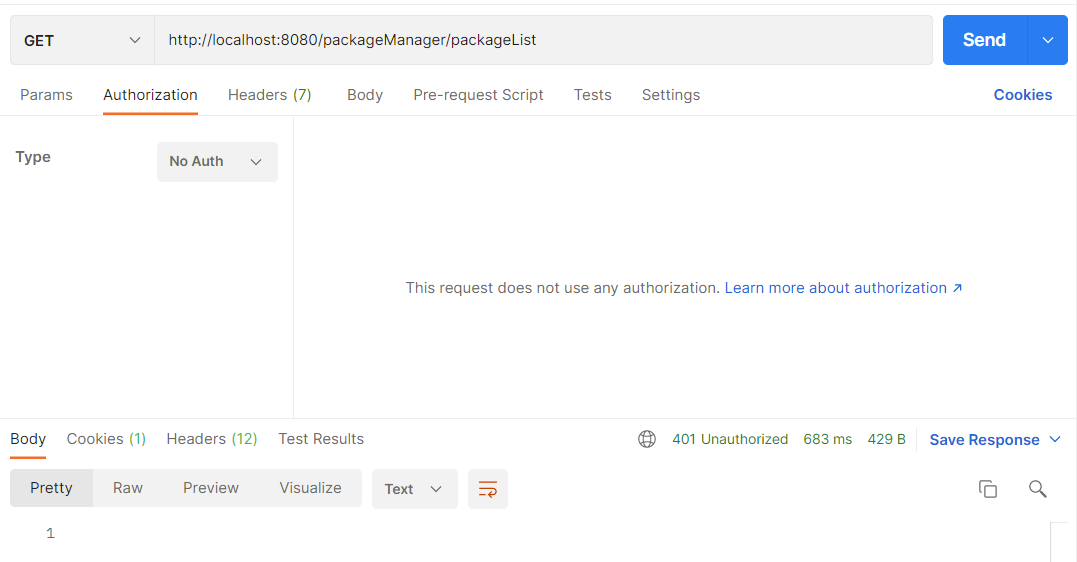
\includegraphics[width=\textwidth]{images/security-postman-1.png}
	\caption{Sending API request without auth}
	\label{ssec:send-api-without-auth}
\end{figure}

\begin{figure}[H]
	\centering
	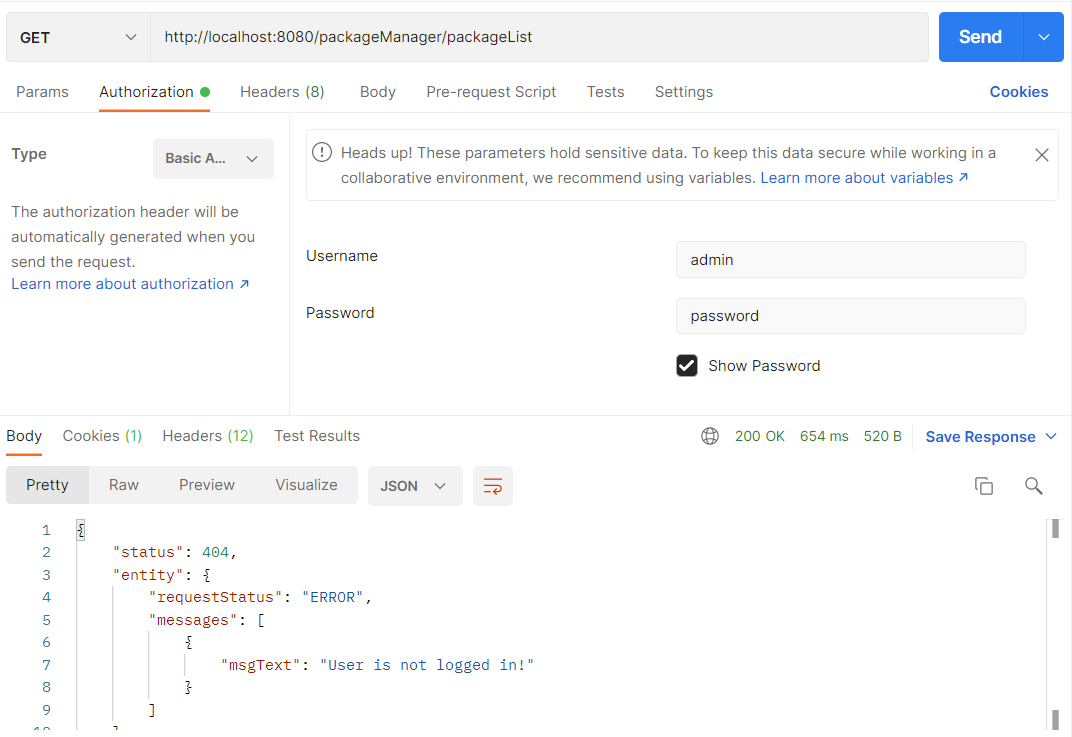
\includegraphics[width=\textwidth]{images/security-postman-2.png}
	\caption{Sending API request with auth}
	\label{ssec:send-api-with-auth}
\end{figure}


\section{Testing}
\label{sec:testing}

Testing is one of the essential parts of the application to prove its correctness against multiple inputs for various API requests. Testing has been divided into 3 files under \texttt{src/test/java/com/ericsson/packageManager} folder. 72 integration tests have been written in order to check if each of the Package, Resource, and User models work correctly and synchronously. Integration tests are written with the Spring MVC framework. 

\subsection{Spring MVC}
Integration testing plays a crucial role in the application development cycle by confirming the end-to-end behavior of a system. Without explicitly starting a Servlet container, the Spring MVC test framework allows the developer to write and run integration tests that test controllers. \texttt{MockMVC} class is part of the Spring MVC test framework. It will be used alongside Spring boot’s \texttt{WebMvcTest} class to execute Junit test cases which check REST controller methods.

\subsection{Test configuration}
First and foremost, the dependency must be included in the \texttt{pom.xml}.
\lstset{caption={Spring Boot Test dependency}, label=src:test-dependency}
\begin{lstlisting}[language={xml}]
<dependency>
  <groupId>org.springframework.boot</groupId>
  <artifactId>spring-boot-starter-test</artifactId>
</dependency>
\end{lstlisting}

A \texttt{JUnit} test class can be utilized with the below-given configuration to test the Spring MVC controller requests and responses.

\lstset{caption={\texttt{UserApiTest} class configuration}, label=src:UserApiTest-class}
\begin{lstlisting}[language={JAVA}]
@RunWith(SpringRunner.class)
@WebMvcTest
@AutoConfigureMockMvc
public class UserApiTest {

    @MockBean
    private UserService userService;

    @MockBean
    private StorageService storageService;

    @MockBean
    private PackageService packageService;

    @MockBean
    private ResourceService resourceService;

    @Autowired
    PackageManagerController packageManagerController;

    @Autowired
    private MockMvc mockMvc;
    //
}
\end{lstlisting}

\begin{itemize}
    \item \texttt{SpringRunner} is an alias for the \texttt{SpringJUnit4ClassRunner}. This is used for providing \texttt{Spring TestContext Framework} functionality which will support annotations and classes. It is a custom extension of JUnit’s \texttt{BlockJUnit4ClassRunner}.
    \item \texttt{@WebMvcTest} annotation is used for Spring MVC tests. It impairs full auto-configuration, but applies configuration relevant to MVC tests.
    \item The \texttt{WebMvcTest} annotation auto-configure \texttt{MockMvc} instance as well.
    \item  \texttt{@MockBean} annotation add mock objects to the Spring application context. This mock is replacing any existing bean of the same type in the application context
\end{itemize}

\subsubsection{Post and Put requests testing}
In this code snippet below, a POST request with URL has been performed which has content JSON. After request performed out, \texttt{Matchers} are checked based on the parameter given such as \texttt{code}, \texttt{requestStatus} and \texttt{messages}. Whole data as JSON parameter is assigned to \texttt{result} variable. This helps us to check all the messages one by one. When it comes to the PUT request, it is the same as POST, \texttt{MockMvcRequestBuilders.put(url)} is the only difference that needs to be changed.
\lstset{caption={POST Request Testing}, label=src:post-request-method}
\begin{lstlisting}[language={JAVA}]
MvcResult result = mockMvc.perform(MockMvcRequestBuilders.post(url)
    .header(HttpHeaders.AUTHORIZATION,"Basic " + Base64Utils.encodeToString("admin:password".getBytes()))
    .content(content)
    .contentType(MediaType.APPLICATION_JSON))
    .andExpect(MockMvcResultMatchers.status().isOk())
    .andExpect(MockMvcResultMatchers.jsonPath("$.status", Is.is(code)))
    .andExpect(MockMvcResultMatchers.jsonPath("$.entity.requestStatus", Is.is(requestStatus)))
    .andExpect(MockMvcResultMatchers.jsonPath("$.entity.messages").isArray())
    .andExpect(MockMvcResultMatchers.jsonPath("$.entity.messages", hasSize(messages.size())))
    .andExpect(MockMvcResultMatchers.content().contentType(MediaType.APPLICATION_JSON)).andReturn();
        
List<String> expectedMessages = new ArrayList<>();
for(int i = 0; i < messages.size(); i++){
    String path = "$.entity.messages[" + i + "].msgText";
    expectedMessages.add(JsonPath.read(result.getResponse().getContentAsString(), path));
}
for (String s : messages) {
    assertThat(expectedMessages, hasItem(s));
}
\end{lstlisting}

\subsubsection{Delete Requests Testing}
Testing the DELETE requests is the same as the POST request mentioned above. The only difference is that there is no JSON content to add to the header.

\lstset{caption={DELETE Request Testing}, label=src:delete-request-method}
\begin{lstlisting}[language={JAVA}]
mockMvc.perform(MockMvcRequestBuilders.delete(url)
    .header(HttpHeaders.AUTHORIZATION,"Basic " + Base64Utils.encodeToString("admin:password".getBytes())))
    .andExpect(MockMvcResultMatchers.status().isOk())
    .andExpect(MockMvcResultMatchers.jsonPath("$.status", Is.is(code)))
    .andExpect(MockMvcResultMatchers.jsonPath("$.entity.requestStatus", Is.is(requestStatus)))
    .andExpect(MockMvcResultMatchers.jsonPath("$.entity.messages").isArray())
    .andExpect(MockMvcResultMatchers.jsonPath("$.entity.messages", hasSize(1)))
    .andExpect(MockMvcResultMatchers.jsonPath("$.entity.messages[0].msgText", Is.is(message)))
    .andExpect(MockMvcResultMatchers.content().contentType(MediaType.APPLICATION_JSON));

\end{lstlisting}

\subsubsection{Get Requests Testing}
As we already know, the response coming from GET request is divided into 2 types. When it is successful, the response is the list of requested objects such as Packages, Users. After getting resulted variable, objects are examined. Otherwise, the usual error response which is mentioned in~\autoref{subsubsec:response-body-structures} appears and it is handled as the previous requests.

\lstset{caption={GET Request Testing Success Response}, label=src:get-request-method-1}
\begin{lstlisting}[language={JAVA}]
MvcResult result = mockMvc.perform(MockMvcRequestBuilders.get(url)
    .header(HttpHeaders.AUTHORIZATION,"Basic " + Base64Utils.encodeToString("admin:password".getBytes())))
    .andExpect(MockMvcResultMatchers.status().isOk())
    .andExpect(MockMvcResultMatchers.content().contentType(MediaType.APPLICATION_JSON)).andReturn();
        //
\end{lstlisting}

\lstset{caption={GET Request Testing Failure Response}, label=src:get-request-method-2}
\begin{lstlisting}[language={JAVA}]
mockMvc.perform(MockMvcRequestBuilders.get(url)
    .header(HttpHeaders.AUTHORIZATION,"Basic " + Base64Utils.encodeToString("admin:password".getBytes())))
    .andExpect(MockMvcResultMatchers.status().isOk())
    .andExpect(MockMvcResultMatchers.jsonPath("$.status", Is.is(code)))
    .andExpect(MockMvcResultMatchers.jsonPath("$.entity.requestStatus", Is.is(requestStatus)))
    .andExpect(MockMvcResultMatchers.jsonPath("$.entity.messages").isArray())
    .andExpect(MockMvcResultMatchers.jsonPath("$.entity.messages", hasSize(1)))
    .andExpect(MockMvcResultMatchers.jsonPath("$.entity.messages[0].msgText", Is.is(message)))
    .andExpect(MockMvcResultMatchers.content().contentType(MediaType.APPLICATION_JSON));
\end{lstlisting}

\subsection{Testing results}

In conclusion, with the help of the Spring MVC test framework, all the edge cases of possible API requests have been checked. All of the 72 integration tests in 3 different test classes passed the verification. See~\autoref{ssec:packageapitest-class},~\autoref{ssec:resourcecapitest-class}, and~\autoref{ssec:userapitest-class}. 

Using template methods for different HTTP request types made it easier and quicker to write effective test cases. All of the successful tests proved that our application can run smoothly without any errors and exceptions.

\begin{figure}[H]
	\centering
	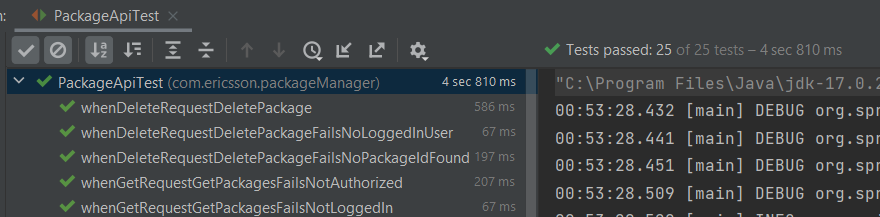
\includegraphics[width=150mm]{images/successful-tests.png}
	\caption{\texttt{PackageApiTest} test class result}
	\label{ssec:packageapitest-class}
\end{figure}

\begin{figure}[H]
	\centering
	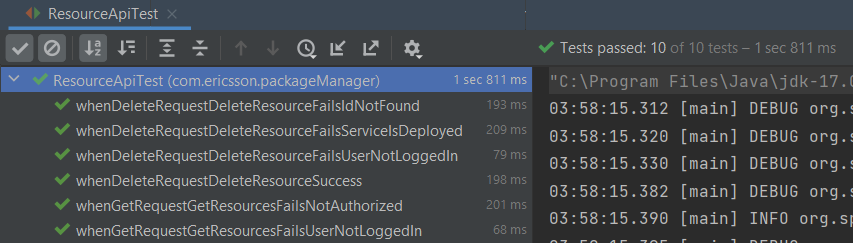
\includegraphics[width=150mm]{images/resource-api-tests.png}
	\caption{\texttt{ResourceApiTest} test class result}
	\label{ssec:resourcecapitest-class}
\end{figure}

\begin{figure}[H]
	\centering
	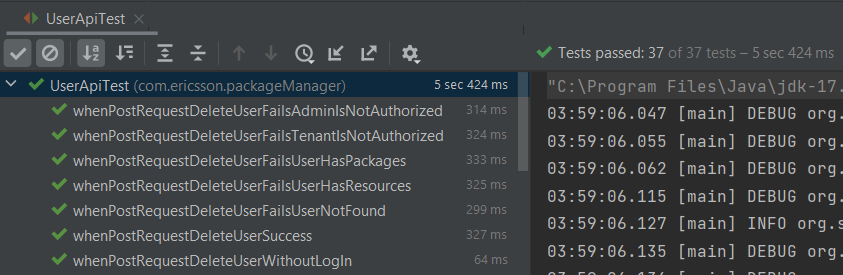
\includegraphics[width=150mm]{images/user-api-tests.png}
	\caption{\texttt{UserApiTest} test class result}
	\label{ssec:userapitest-class}
\end{figure}

The implementation and testing phases were explained in this chapter. Now it is time to move to the conclusion to explain what I have gained through this project and possible additional work in the future.
